\chapter{REQUIREMENTS ANALYSIS}
\label{chap:requirements}

\section{Biopotential Electrodes}
Biopotential electrodes are used to measure small electrical signals produced inside the human body. These signals come from active cells such as brain cells and muscle cells. In EEG systems, two electrodes are used for each channel to measure the changing voltage on the scalp. This can be done by measuring the voltage between two points on the head, called bipolar configuration, or between one point on the head and a reference point like the ear, called unipolar configuration \cite{malmivuo1995bioelectromagnetism}.

Biopotential electrodes are mainly divided into two types: wet electrodes and dry electrodes. Wet EEG electrodes are usually small cup shaped electrodes filled with conductive gel. The gel helps the electrode make good contact with the scalp, even through hair. Dry electrodes do not use gel. Instead, they have small teeth like structures that pass through the hair and touch the scalp directly.

The problem with wet electrodes is that the gel can dry out affecting the signal quality and and it also causes skin irritaiton in some patients. Dry electrodes are generally more comfortable and easier to use because they do not require gel. However, they are more affected by body movement and usually have higher resistance between the skin and the electrode \cite{saab2011drywet}.

\begin{figure}[htbp]
	\centering
	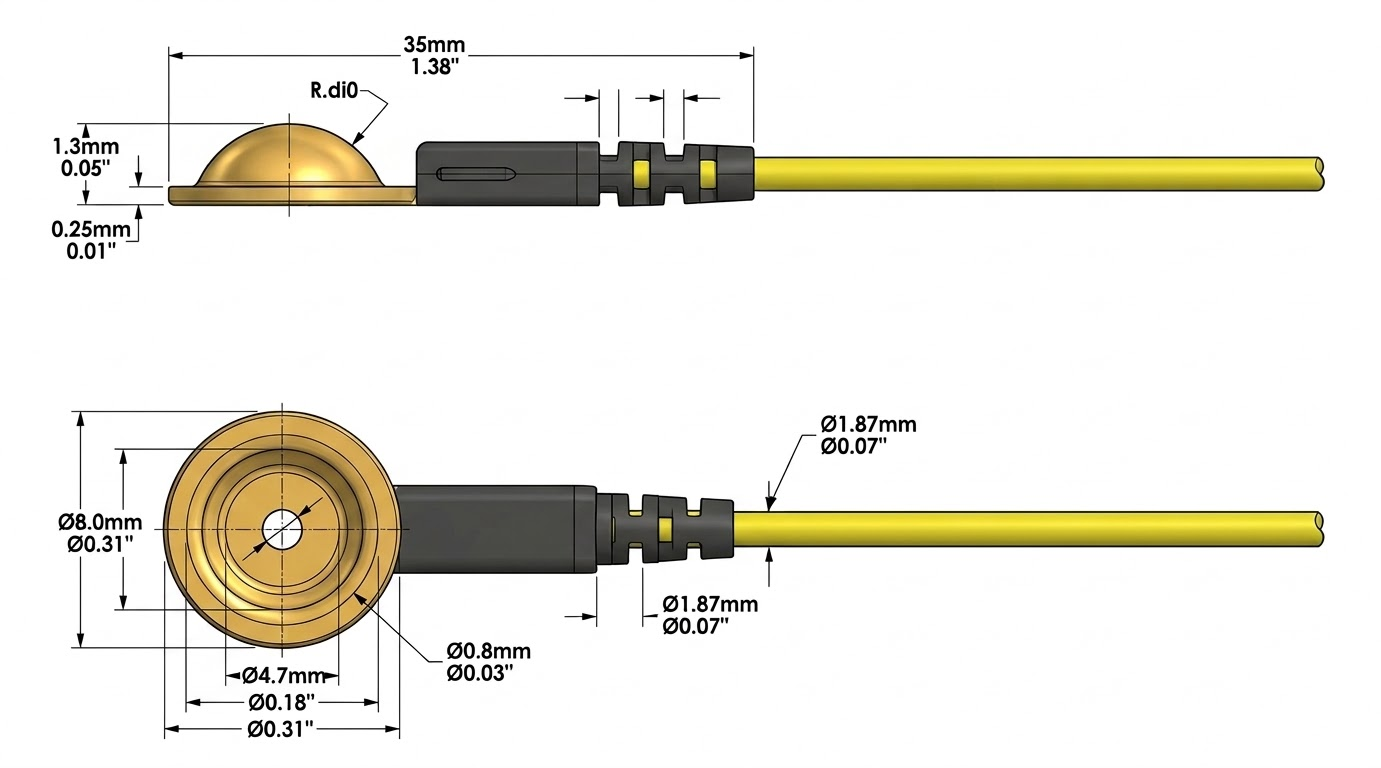
\includegraphics[width=0.45\textwidth]{src/images/figures/wet_cup_electrodes.png}
	\caption{\centering Wet EEG cup electrodes}
	\label{fig:wetElectrodes}
\end{figure}

EEG electrodes can also be made from different materials, such as silver/silver chloride, gold, silver, stainless steel, and tin. Reusable EEG electrodes are often expensive and can cost ten dollars or more per electrode \cite{biomedical2018electrodes}. To reduce the overall cost of the project, low cost and homemade electrodes were used.

Another way to classify EEG electrodes is as active or passive. Active electrodes include a small amplifier near the electrode itself. This helps reduce noise caused by poor contact with the skin and movement of wires \cite{gtec2018comparison}. Passive electrodes do not have this amplifier and are connected directly to the bio signal amplifier using long wires.


\section{Instrumentation Amplifier}
An instrumentation amplifier is used to amplify very small EEG signals obtained from the scalp electrodes. Brain signals are very weak and cannot be directly processed by filters or other circuits. Therefore, an instrumentation amplifier is used as the first stage of signal conditioning in this project.

In this system, the AD620 instrumentation amplifier is used because it is specially designed for low level bio potential signal amplification such as EEG. AD620 has high input impedance, which prevents loading of the electrodes and helps maintain signal quality. It also has high common mode rejection, which reduces common mode noise such as power line interference and motion artifacts.

\begin{figure}[H]
	\centering
	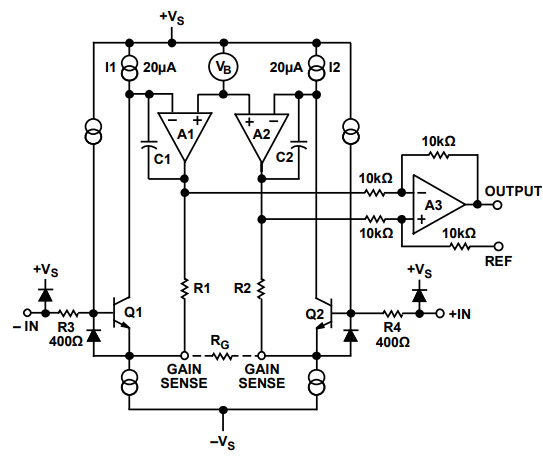
\includegraphics[width = 14cm]{src/images/figures/ad620_schematic.png}
	\caption{\centering Simplified Schematic of AD620 Source: \cite{ad620datasheet}}
\end{figure}

The gain of AD620 can be easily adjusted using a single external resistor, which makes the circuit simple and flexible. AD620 also operates with low noise, low power
consumption, and stable performance, making it suitable for continuous EEG signal acquisition.

By using the AD620 instrumentation amplifier, the small voltage difference between EEG electrodes is amplified accurately while rejecting common noise signals. This
improves signal clarity and makes the EEG signal suitable for further filtering and processing in the Brain-Computer Interface system.

\section{Types of Filters}
The role of filters in the EEG system is to remove noise and only allow the desired signals to be detected. The signals in the EEG are quite weak and susceptible to any noise. Some of the noises that can affect the EEG signals include power line interference and muscle movements among others. Therefore, the use of filters in signal conditioning is quite crucial.

Band pass filter is one of the filters used in the current project. In the case of band pass filter, only the required frequency of the EEG is allowed to pass through the filter. It eliminates slow drift and high frequency noises from the signal.

Low pass filter is used to eliminate high frequency noise. The high frequency noise includes muscle activity and external electrical interference.

High pass filter is employed in order to get rid of very low frequency noise. These kinds of noises include body movements and baseline drift.

In the current project, simple analog filters are used. They are simple to design and therefore suitable for low cost systems. They eliminate enough noise in order to detect eye blink and basic EEG frequencies.

\section{Arduino Microcontroller}
When the signal from the electrodes is converted into digital form, the microcontroller takes the samples and processes them within small time intervals. The initial signal processing functions such as amplitude thresholding are performed in the time domain. In order to perform frequency domain analysis, the microcontroller applies Fast Fourier Transform (FFT) algorithm on the digital EEG signal. As the result of the FFT analysis, the microcontroller detects eye blinks because eye blinks produce low frequencies.

In case of receiving valid brain or eye blink commands, the microcontroller uses predefined algorithms to make decisions and produces corresponding output signals. The outputs generated by the microcontroller can be used to control external devices like a cursor, virtual keyboard, or LED lights. Moreover, the microcontroller manages data communication between a computer or display device and the microcontroller. Therefore, the microcontroller is responsible for performing data acquisition, signal processing, decision making, and controlling devices within the BCI project.

\section{FFT and MATLAB (Signal Processing and Visualization)}
Fast Fourier Transform (FFT) is adopted in this work to transform the input EEG signal from time domain to frequency domain since frequency domain analysis is necessary to distinguish and extract certain frequency bands in the EEG signal, especially the beta band (12-30 Hz) that is related to relaxation and attention.

EEG signals obtained from Arduino are analyzed in MATLAB in which FFT is implemented to compute the power spectral density of the input signal. Depending on the strength of the beta band in the EEG signals, the mental state of the user can be determined.

MATLAB plotting tools can be used to plot the time domain signal as well as the frequency spectrum of the input EEG signals. This will facilitate performance analysis and validation of the implemented signal processing techniques.
